\begin{framed}

Objetivos:
\begin{itemize}
    \item Estudiar la superposición de flujos potenciales. 
\end{itemize}

Contenidos:
\begin{itemize}
    \item Repaso de flujos elementales.
    \item El principio de superposición en la ecuación de Laplace. 
    \item Ejemplos de aplicación
    \begin{itemize}
        \item El cuerpo de Rankine. 
        \item Flujo alrededor de un cilindro. 
    \end{itemize}
\end{itemize}

Bibliografía:
\begin{itemize}
    \item White, F. M. (2008) Mecánica de Fluidos. McGraw-Hill. Sexta edición. Secciones 4.10
    \item Fox, R. W., Pritchard, P. J. y McDonald, A. T. (2009) Introduction to Fluid Mechanics. John Wiley \& Sons. Sección 6.7.
\end{itemize}
\end{framed}

\section*{Flujos elementales}

La clase pasada estudiamos flujos potenciales elementales.
Estos son, básicamente, soluciones analíticas de la ecuación de Laplace (con un $\delta$ de Dirac en algunos casos) con condiciones de contorno que tienen sentido físico.
Para el caso de los flujos elementales que estudiamos, la condición de que usamos es de velocidad hacia el infinito, que era $U_\infty$ en el flujo uniforme, y cero en los vórtices, fuente, sumidero y dobletes.
Sin embargo, no hay que confundirse: cualquier solución de la ecuación de Laplace que cumpla con condiciones de borde físicas representa el movimiento de un flujo ideal.
De hecho, hoy vamos a encontrar más soluciones de flujo potencial.

Solo como recordatorio de la clase pasada, los flujos elementales son:

\begin{itemize}
\item Flujo uniforme horizontal (dirección $+x$):
\begin{align}
u &= U_\infty \quad v = 0 \nonumber \\
\phi&= U_\infty x \quad \psi= U_\infty y
\end{align}

\item Flujo uniforme vertical (dirección $+y$):
\begin{align}
u &= 0 \quad v = V_\infty \nonumber \\
\phi&= V_\infty y \quad \psi= -V_\infty x
\end{align}

\item Fuente:
\begin{align}
V_r &= \frac{q}{2\pi r}\quad V_\theta=0\nonumber\\
\phi&=\frac{q}{2\pi}\ln(r) \quad \psi=\frac{q}{2\pi}\theta
\end{align}

\item Sumidero:
\begin{align}
V_r &= -\frac{q}{2\pi r}\quad V_\theta=0\nonumber\\
\phi&=-\frac{q}{2\pi}\ln(r) \quad \psi=-\frac{q}{2\pi}\theta
\end{align}

\item Vórtice (dirección contra reloj):
\begin{align}
V_r &= 0 \quad V_\theta=\frac{\Gamma}{2\pi r}\nonumber\\
\phi&=\frac{\Gamma}{2\pi}\theta \quad \psi = -\frac{\Gamma}{2\pi}\ln(r).
\end{align}

\item Doblete: 
\begin{align}
V_r = -K\frac{\cos(\theta)}{r^2}\quad V_\theta = -K\frac{\sin(\theta)}{r^2}\nonumber\\
\phi=K\frac{\cos(\theta)}{r}\quad \psi = -K\frac{\sin(\theta)}{r}.
\end{align}

\end{itemize}

\section*{Principio de superposición}
Sabemos que para flujos ideales tanto $\phi$ como $\psi$ satisfacen la ecuación de Laplace.
La ecuación de Laplace es homogenea (todos los términos de la ecuación contienen la variable dependiente) y lineal (la variable dependiente no está elevada a una potencia), por lo tanto, si $\phi_1$ y $\phi_2$ satisfacen la ecuación de Laplace, $\phi_3=\phi_1+\phi_2$ también es una solución.
Si aterrizamos esto al caso de flujo potencial, podríamos decir que $\mathbf{V}_3=\mathbf{V}_1+\mathbf{V}_2$, además $\psi_3=\psi_1+\psi_2$.
Esta propiedad nos permite combinar soluciones simples de flujo potencial, como los flujos elementales, para modelar flujos más interesantes, con aplicaciones reales.
De hecho, esta ya lo hicimos sin darnos cuenta en la derivación del doblete: sumamos la solución de una fuente y un sumidero.
En esta clase, vamos a revisar algunas soluciones con superposición que son relevantes en mecánica de fluidos.

Algo que no hemos discutido en profundidad todavía, y que hoy tomará importancia, es la interpretación de líneas de flujo como cuerpos sólidos.
La característica de las líneas de flujo es que la velocidad es tangencial a ellas, por lo tanto, no existe flujo ``a través'' de una línea de flujo.
Por otra parte, al ser este un flujo no viscoso, la condición de contorno correspondiente es la de impermeabilidad (flujo no pasa a través de un sólido, $\mathbf{V}\cdot\mathbf{n}=0$), pero si puede resbalar por él.
Si se fijan, la condición de borde de impermeabilidad es equivalente a una línea de flujo, por lo que podemos mirar a una línea de flujo como un cuerpo sólido.
Vamos a revisitar esto en los ejemplos que veremos a continuación, y les quedará mucho más claro.

\subsection*{Cuerpo de Rankine}

El cuerpo de Rankine es de los flujos superpuestos más simples, en donde se suma un flujo uniforme con una fuente.
En este caso, conviene pasar las ecuaciones de flujo uniforme a coordenadas polares, dejándonos
%
\begin{equation}
\phi_U = U_\infty r\cos(\theta) \quad \psi_U = U_\infty r\sin(\theta).
\end{equation}
%
Por lo tanto, la función potencial y corriente del cuerpo de Rankine es
%
\begin{align}\label{eq:rankine}
\phi_R &= \phi_U+\phi_f = U_\infty r\cos(\theta) + \frac{q}{2\pi}\ln(r)\nonumber\\
\psi_R &= \psi_U+\psi_f = U_\infty r\sin(\theta) + \frac{q}{2\pi}\theta,
\end{align}
%
y podemos calcular la velocidad al sacar la grandiente del potencial ($\nabla\phi$)
%
\begin{align}\label{eq:rankine_vel}
V_r = \frac{\partial\phi}{\partial r} = U_\infty\cos(\theta) + \frac{q}{2\pi r} \nonumber\\
V_\theta = \frac{1}{r}\frac{\partial\phi}{\partial\theta} = -U_\infty\sin(\theta)
\end{align}

\paragraph{Ejemplo.}
Sumemos un flujo uniforme con $U_\infty=1$ con una fuente con caudal $q=5$ y grafiquemos sus líneas de flujo.
Viendo la Ec. \eqref{eq:rankine}, la función corriente sería
%
\begin{equation}\label{eq:rankine_ej}
\psi_R = r\sin(\theta)+\frac{1}{2\pi}\theta.
\end{equation}
%
Esta solución está graficada en la Figura \ref{fig:rankine}
%
\begin{figure}[h!]
\centering
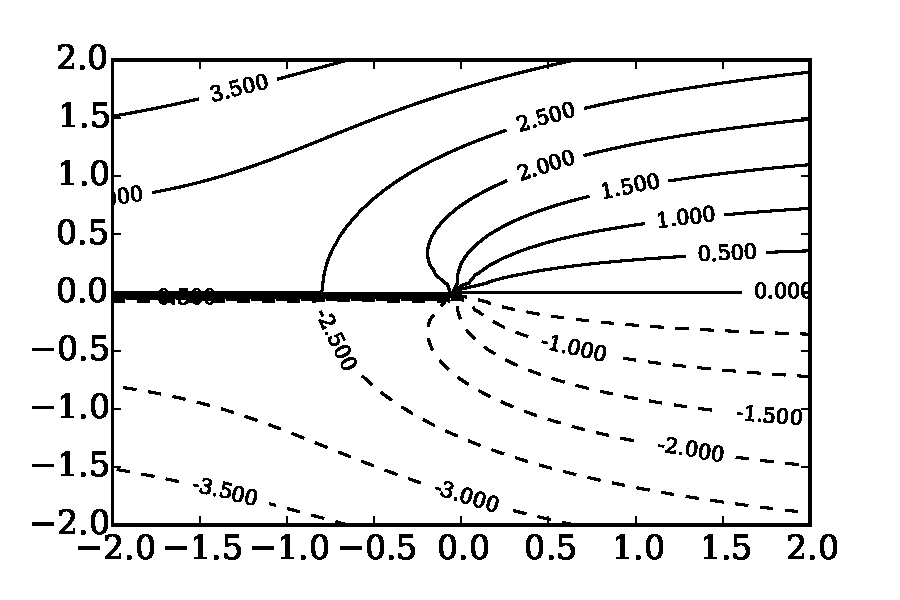
\includegraphics[width=0.7\textwidth]{clase11/rankine.pdf}
\caption{Cuerpo de Rankine}
\label{fig:rankine}
\end{figure}

Un punto de interés de esta suma entre flujo uniforme y fuente es que debe haber un punto de velocidad $\mathbf{V}=0$ sobre el eje $x$; busquemos ese punto.
Sobre el eje $x$ la componente $V_\theta$ debe ser 0 (por simetría), y $\theta=\phi$.
Reemplazando esos valores en la Ec. \eqref{eq:rankine_vel}, llegamos a
%
\begin{align}
V_r = 1\cos(\pi) + \frac{5}{2\pi r} &= 0\nonumber\\
\Rightarrow r &= 2\pi.
\end{align}
%
Entonces, existe un punto de estancamiento en $r=2\pi, \theta=\pi$.

Fíjense más de cerca en la Figura \ref{fig:rankine}: parece ser que tenemos dos regiones, una dentro y otra afuera de la línea de flujo con $\psi=2.5$. 
Reemplacemos la ubicación del punto de estancamiento en $\psi_R$ de la Ec. \eqref{eq:rankine_ej}:
%
\begin{equation}
\psi_R(r=2\pi,\theta=\pi) = 2\pi\sin(\pi)+\frac{5}{2\pi}\pi = 2.5
\end{equation}
%
la línea que divide las dos regiones pasa exactamente por el punto de estancamiento! 
Esto nos indica que la línea de flujo $\psi=2.5$ puede ser vista como un sólido enfrentado a un flujo: es el cuerpo de Rankine.
La región fuera de la línea $\psi=2.5$ pasa alrededor del cuerpo de Rankine, mientras que lo que está adentro se puede considerar dentro del sólido.
Aquí hay una aplicación de la interpretación de una línea de flujo como un sólido, ya que genera un punto de estancamiento, y sabemos que la velocidad nunca tendra una componente normal a éste, por lo que el flujo nuna lo atravesará.

\subsection*{Flujo alrededor de un cilindro}
La suma de un doblete y un flujo uniforme entrega un lo que se conoce como flujo alrededor de un cilindro.
La función potencial y corriente da:
%
\begin{align}\label{eq:cilindro_pot}
\phi_c &= \phi_U+\phi_d = U_\infty r\cos(\theta) + K\frac{\cos(\theta)}{r}\nonumber\\
\psi_c &= \psi_U+\psi_d = U_\infty r\sin(\theta) - K\frac{\sin(\theta)}{r}
\end{align}
%
y sacando el gradiente podemos obtener la velocidad:
%
\begin{align}\label{eq:cilindro_vel}
V_r = \frac{\partial\phi}{\partial r} = U_\infty\cos(\theta) - K\frac{\cos(\theta)}{r^2} \nonumber\\
V_\theta = \frac{1}{r}\frac{\partial\phi}{\partial\theta} = -U_\infty\sin(\theta) - K\frac{\sin(\theta)}{r^2}
\end{align}

\paragraph{Ejemplo.} 
Sumemos a un flujo uniforme con $U_\infty$ un doblete con $K=1$.
La ecuación de la función corriente queda:
%
\begin{equation}\label{eq:cilindro_ej}
\psi_c =  1 r\sin(\theta) - 1\frac{\sin(\theta)}{r}
\end{equation}
%
y la figura \ref{fig:cilindro} muestra sus curvas de nivel ($\psi=$constante) gráficamente.
%
\begin{figure}[h!]
\centering
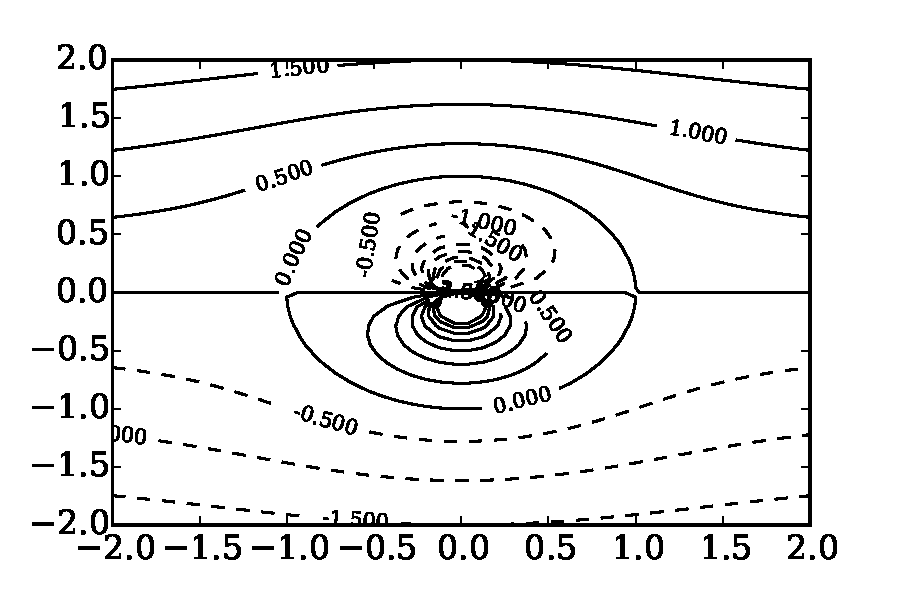
\includegraphics[width=0.7\textwidth]{clase11/cilindro.pdf}
\caption{Flujo alrededor de un cilindro}
\label{fig:cilindro}
\end{figure}

Viendo la Figura \ref{fig:cilindro} se hace patente por qué se le conoce como flujo alrededor de un cilindro: el flujo se divide en dos zonas: el flujo externo y lo que está encerrado por el cículo con $\psi=0$.
De la experiencia con el cuerpo de Rankine, podemos suponer que ese círculo con $\psi=0$ puede representar a un sólido; veamos si se genera un punto de estancamiento en él.
Por simetría, podemos intuir que el punto de estancamiento se encuentra sobre el eje $x$, en el lado izquierdo del cilindro, donde se enfrenta con el flujo ($\theta=\pi$).
Sobre el eje $x$, no hay componente $\theta$ de la velocidad, y queremos encontrar $r$ tal que la velocidad sea $0$:
%
\begin{align}
V_r = 1\cos(\pi) - 1\frac{\cos(\pi)}{r^2} =0 \nonumber\\
\Rightarrow r = 1.
\end{align}
%
Justamente, si reemplazamos $r=1, \theta=\pi$ en la Ec. \eqref{eq:cilindro_ej}, llegamos a $\psi_c=0$, cosa que habíamos intuído gráficamente de la Figura \ref{fig:cilindro}.
Además, podemos darnos cuenta que hay otro punto de estancamiento en $r=1, \theta=0$. 

Generalicemos esto a cualquier $U_\infty$ y $K$.
En el caso general, el punto de estancamiento estaría en:
%
\begin{align}
V_r = U_\infty\cos(\pi) - K\frac{\cos(\pi)}{r^2} &=0 \nonumber\\
\Rightarrow r &= \sqrt{\frac{K}{U_\infty}}
\end{align}
%
por lo tanto, la curva de nivel que delimita al cilindro se obtiene reemplazando $\theta=\pi,r=\sqrt{K/U_\infty}$ en la Ec. \eqref{eq:cilindro_pot}
%
\begin{align}
\psi_c &= U_\infty \sqrt{\frac{K}{U_\infty}}\sin(\theta) - K\frac{\sin(\theta)}{\sqrt{\frac{K}{U_\infty}}}\nonumber\\
\psi_c&=\sqrt{U_\infty K}\sin(\theta)-\sqrt{U_\infty K}\sin(\theta)=0.
\end{align}
%
Así, podemos ver que el cilindro siempre estará delimitado por la curva $\psi_c=0$.

Verifiquemos que realmente se trata de un cilindro.
Sabemos que el sólido está delimitado por la curva $\psi_c=0$, que es:
%
\begin{align}
\psi_c &= U_\infty r\sin(\theta) - K\frac{\sin(\theta)}{r} = 0\nonumber\\
&U_\infty\sin(\theta)r\left(1-\frac{K}{U_\infty r^2}\right) = 0\nonumber\\
&\Rightarrow r=\sqrt{\frac{K}{U_\infty}}.
\end{align}
%
La curva $r=\sqrt{K/U_\infty}$ en coordenadas polares representa un círculo con radio $r=\sqrt{K/U_\infty}$, confirmándonos que es un cilindro circular.
Si no están tan familiarizados con las coordenadas polares pueden transformar a coordenadas cartesianas, donde $r=\sqrt{x^2+y^2}$:
%
\begin{equation}
r^2=x^2+y^2=\frac{K}{U_\infty}.
\end{equation}

\paragraph{Velocidad en la superficie del cilindro.}
La línea de flujo $\psi_c=0$ es un círculo por el cual no atraviesa flujo, pues la velocidad es tangente.
Ya que es un círculo, la componente radial de la velocidad debe ser cero.
Por otra parte, desde la Ec. \eqref{eq:cilindro_vel}, la velocidad angular sobre la superficie del cilindro es
%
\begin{equation}
V_c = -U_\infty\sin(\theta) - K\frac{\sin(\theta)}{\frac{K}{U_\infty}} = -2U_\infty\sin(\theta).
\end{equation}
%
lo que nos confirma que hay dos puntos de estancamiento (en $\theta=\pi$ y $\theta=0$).
Además nos podemos dar cuenta que el punto de máxima velocidad es la parte superior e inferior del cilindro ($\theta=\pi/2$ y $\theta=3\pi/2$), donde la velocidad es el doble de la velocidad al infinito.
Sobre el eje $y$ ($\theta=\pi/2$) la velocidad no tiene componente radial (por simetría), así es que, a medida que nos alejamos de la superficie del cilindro, la velocidad debe variar desde $2U_\infty$ a $U_\infty$ de la forma
%
\begin{equation}
V_\theta = -U_\infty - \frac{K}{r^2}
\end{equation}

\paragraph{Presión alrededor del cilindro.}

Revisitemos sus conocimientos de mecánica de fluidos general.
La ecuación de Bernoulli es válida para flujos incompresibles y no viscosos (es una integración de la ecuación de Euler), que es exactamente la situación en flujo potencial.
Despreciando el efecto de la diferencia de altura (que de hecho se cancela), podemos aplicar la ecuación de Bernoulli entre un punto al infinito (donde $\mathbf{V}=U_\infty$ y $p=p_\infty$) para llegar a una expresión de presión en la superficie del cilindro:
%
\begin{align}\label{eq:cilindro_p}
&\frac{p_\infty}{\rho} + \frac{U_\infty^2}{2} = \frac{p_c(\theta)}{\rho} + \frac{V_c^2}{2}\nonumber\\
&p(\theta) = \frac{\rho}{2}\left(U_\infty^2-V_c^2\right) + p_\infty = \frac{U_\infty^2\rho}{2}\left(1+4\sin^2(\theta)\right) + p_\infty
\end{align}

Usemos la Ec. \eqref{eq:cilindro_p} para encontrar la fuerza que está resistiendo el cilindro.
Si hacemos un volúmen de control justo por el contorno del cilindro, no hay flujo que entre al volumen de control y la única fuerza presente es la que la presión hace sobre el contorno del volúmen de control.
Esta fuerza es siempre normal a la superficie y con dirección opuesta a la normal $\mathbf{n}$ que sale del cilindro, la cual es equivalente a un vector unitario $\mathbf{r}/|\mathbf{r}|$ en dirección radial (ver Figura \ref{fig:presion_cilindro}).
%
\begin{figure}[h!]
\centering
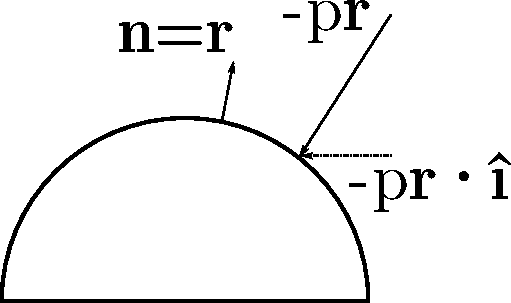
\includegraphics[width=0.5\textwidth]{clase11/presion_cilindro.pdf}
\caption{Presión alrededor del cilindro}
\label{fig:presion_cilindro}
\end{figure}

Integremos la Ec. \eqref{eq:cilindro_p} sobre toda la superficie del cilindro para encontrar la componente $x$ de la fuerza.
%
\begin{align}\label{eq:fuerza_x}
&F_x = \oint_A -p\mathbf{n}dS\cdot\ihat = -\oint_A p\mathbf{r}\cdot\ihat Rd\theta \nonumber\\
&\mathbf{r}\cdot\ihat =\frac{r_x}{R} \text{, donde, } r_x = R\cos(\theta),
\end{align}
%
donde $R$ es el radio del cilindro, $\mathbf{r}=(r_x,r_y)$ es en este caso la superficie del cilindro, y un elemento de superficie es $dS-Rd\theta$.
Si usamos la Ec. \eqref{eq:cilindro_p}, llegamos a
%
\begin{align}
F_x = -\int_0^{2\pi}\left[\frac{U_\infty^2\rho}{2}(1+4\sin^2(\theta))+p_\infty\right]R\cos(\theta)d\theta=0.
\end{align}
El primer y segundo término son la integral $\int_0^{2\pi}\cos(\theta)d\theta=0$.
El segundo término es $\int_0^{2\pi}\sin^2\theta\cos\theta d\theta=0$, lo cual es fácil de demostrar al reemplazar $u=\sin\theta$.

En conclusión, la componente $x$ de la fuerza es $F_x=0$, lo cual va totalmente contra la intuición: si viene un flujo sobre un cuerpo \mbox{?`}no debiese empujarlo? En un flujo ideal, no.
Esto se conoce como la paradoja de D'Alembert, y fue resuelta por Prandtl en 1904, cuando considera la viscosidad. 

\subsection*{Cilindro con circulación}
Al cilindro que ya calculamos en la sección anterior, sumémosle un vórtice de circulación $\Gamma$ que gira en sentido horario:
%
\begin{align}\label{eq:cilindro_circ_pot}
\phi_L &= \phi_U+\phi_d+\phi_v = U_\infty r\cos(\theta) + K\frac{\cos(\theta)}{r} - \frac{\Gamma}{2\pi}\theta \nonumber\\
\psi_L &= \psi_U+\psi_d+\psi_v = U_\infty r\sin(\theta) - K\frac{\sin(\theta)}{r} + \frac{\Gamma}{2\pi}\ln(r)
\end{align}
%
y sacando el gradiente podemos obtener la velocidad:
%
\begin{align}\label{eq:cilindro_circ_vel}
V_r = \frac{\partial\phi}{\partial r} = U_\infty\cos(\theta) - K\frac{\cos(\theta)}{r^2} \nonumber\\
V_\theta = \frac{1}{r}\frac{\partial\phi}{\partial\theta} = -U_\infty\sin(\theta) - K\frac{\sin(\theta)}{r^2} - \frac{\Gamma}{2\pi r}
\end{align}

\paragraph*{Ejemplo.}
Grafiquemos las líneas de flujo de un flujo uniforme con $U_\infty=1$ sumado a un doblete con $K=1$ y un vórtice centrado con $\Gamma=5$.
La ecuación de $\psi_L$ es
%
\begin{equation}
\psi_L = r\sin(\theta) - \frac{\sin(\theta)}{r} + \frac{5}{2\pi}\ln(r)
\end{equation}
%
y sus curvas de nivel están graficadas en la Figura \ref{fig:cilindro_circ}
%
\begin{figure}[h!]
\centering
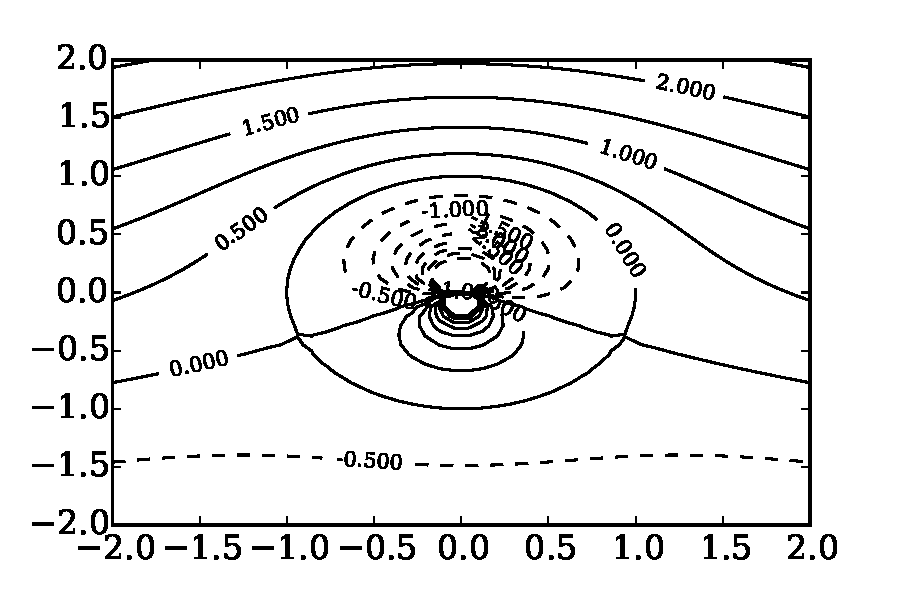
\includegraphics[width=0.7\textwidth]{clase11/cilindro_circ.pdf}
\caption{Cilindro con circulación}
\label{fig:cilindro_circ}
\end{figure}

Miremos la Figura \ref{fig:cilindro_circ} más de cerca.
Es muy parecido al caso anterior, con dos regiones separadas por la línea $\psi_L=0$, sin embargo, los puntos de estancamiento se corrieron hacia abajo!
Pensemos en las implicancias físicas de este hecho; por Bernoulli, sabemos que el punto de menor velocidad es el punto de mayor presión.
Antes, los puntos de estancamiento estaban centrados y en puntos opuestos, pero ahora ambos están en la parte inferior: existe una fuerza neta que empuja al cilindro hacia arriba.

Esto se conoce como el \emph{efecto Magnus}, y existen muchos ejemplos bien domésticos que estoy seguro que han visto (si no, pregúntenle a Fabien Barthez\footnote{\url{https://www.youtube.com/watch?v=XdL7EDKr_rk}})
El efecto Magnus es la base del estudio de la aerodinámica, y la búsqueda de geometrías que puedan volar.
En las clases siguientes vamos a adentrarnos más en estos temas.

\paragraph*{Fuerza de sustentación}
Así como en el cilindro anterior, calculemos la fuerza sobre el cilindro.
Sabemos que la velocidad en la superficie del cilindro tiene solamente componente en $\theta$, por lo tanto, usando la Ec. \eqref{eq:cilindro_circ_vel} en $r=\sqrt{K/U_\infty}$ (el radio del cilindro), obtenemos
%
\begin{align}\label{eq:cilindro_vel_superficie}
V_L &= -U_\infty\sin(\theta) - U_\infty\sin(\theta) - \frac{\Gamma}{2\pi}\sqrt{\frac{U_\infty}{K}}\nonumber\\
V_L &= -2U_\infty\sin(\theta) - \frac{\Gamma}{2\pi}\sqrt{\frac{U_\infty}{K}}.
\end{align}
%
Aplicando Bernoulli entre el infinito y la superficie del cilindro (despreciando efectos de altura), llegamos a:
%
\begin{align}\label{eq:cilindro_circ_p}
p(\theta) &= \frac{\rho}{2}\left(U_\infty^2-V_L^2\right) + p_\infty \nonumber\\
&= \frac{\rho}{2}\left(U_\infty^2+4U_\infty^2\sin^2(\theta) + 2\frac{\Gamma U_\infty}{\pi}\sqrt{\frac{U_\infty}{K}}\sin(\theta) + \left[\frac{\Gamma}{2\pi}\sqrt{\frac{U_\infty}{K}}\right]^2\right) + p_\infty
\end{align}

Diferente a la Ec. \eqref{eq:fuerza_x}, en este caso estamos interesados en calcular la componente $y$ de la fuerza, por lo tanto, la ecuación queda: 
%
\begin{align}\label{eq:fuerza_y}
&F_y = \oint_A -p\mathbf{n}dS\cdot\jhat \text{, con }\mathbf{r}\cdot\jhat =r_y\sqrt{\frac{U_\infty}{K}} \text{ y } r_y = \sqrt{\frac{K}{U_\infty}}\sin(\theta),\nonumber\\
&F_y = -\int_0^{2\pi}\left[p(\theta)\right]\sqrt{\frac{K}{U_\infty}}\sin(\theta)d\theta.
\end{align}
%
La intregral del primer, cuarto y quinto término de la Ec. \eqref{eq:cilindro_circ_p} es básicamente $\int_0^{2\pi}\sin(\theta)d\theta$, cual da cero.
Por otra parte, la integral del segundo término es $\int_0^{2\pi}\sin^3(\theta)d\theta=\int_0^{2\pi}(1-\cos^2(\theta))\sin(\theta)d\theta$, que también da cero (reemplacen $u=cos(\theta)$).
Finalmente, el único término que no se hace cero es el tercero, donde se cancela el $\sqrt{K/U_\infty}$, y es
%
\begin{align}
F_y &= 2\frac{\rho}{2}\frac{\Gamma U_\infty}{\pi}\int_0^{2\pi}\sin^2(\theta)d\theta = \rho\frac{\Gamma U_\infty}{\pi}\int_0^{2\pi}\frac{1}{2}(1-\cos(2\theta))d\theta\nonumber\\
    &= \rho\frac{\Gamma U_\infty}{\pi}\frac{1}{4}(2\theta-\sin(2\theta))_0^{2\pi} = \rho\frac{\Gamma U_\infty}{\pi}\pi = \rho\Gamma U_\infty.
\end{align}

Este resultado nos indica que un cilindro que gira produce una sustentación $L=\rho\Gamma U_\infty$ por unidad de largo.
